\documentclass[12pt]{article}

\usepackage[margin=2cm]{geometry}
\usepackage[T2A]{fontenc}
\usepackage[utf8]{inputenc}
\usepackage[russian]{babel}
\usepackage{multicol}
\usepackage{longtable}
\usepackage{graphics}
\usepackage{rotating}
\usepackage{float}

\setlength{\parindent}{0em}
\setlength{\parskip}{1em}

\usepackage{amsmath, amsfonts, amssymb, amsthm, mathtools}
\usepackage{icomma}

\title{Отчет о выполнении лабораторной работы \\ Определение теплоты испарения жидкости}
\author{Лепарский Роман}
\date{\today}

\begin{document}

\maketitle

\newpage

\section{Аннотация}

\textbf{Цель работы:} 1) измерение давления насыщенного пара жидкости при разной температуре; 2) вычисление по полученным данным теплоты испарения с помощью уравнения Клапейрона–Клаузиуса.

\section{Теоретические сведения}

Испарением называется переход вещества из жидкого в газообразное состояние. Для выхода из жидкости молекулы должны преодолеть силы молекулярного сцепления. Кроме того, при испарении совершается работа против внешнего давления
P. Переход части молекул в пар приводит к обеднению жидкости быстрыми молекулами, т.е. к ее охлаждению.
Количество теплоты, необходимое для изотермического испарения одного моля жидкости при внешнем давлении, равном упругости ее насыщенных паров, называется молярной
теплотой испарения.

В настоящей работе для определения теплоты испарения применен
косвенный метод, основанный на формуле Клапейрона–Клаузиуса:
\begin{equation}
	\frac{dP}{dT} = \frac{L}{T(V_2 - V_1)}
	\label{eq:klapeiron-klausius}
\end{equation}

Найдя из опыта $\frac{dP}{dT}$, $T$, $V_2$ и $V_1$, можно определить $L$ путем расчета. Величины $L$, $V_2$ и $V_1$ в формуле (\ref{eq:klapeiron-klausius}) должны относиться к одному и тому же количеству вещества; мы будем относить их
к одному молю.

Рассмотрим некоторые табличные значения:
\begin{table}[H]
	\centering
	\begin{tabular}{|l|l|l|l|l|l|l|}
		\hline
		& $T_{\text{кип}}$ & $V_1$      & $V_2$      & $b$        & $a$                 & $a/V_2^2$ \\
		Вещество       &                  & $10^{-6}$  & $10^{-3}$  & $10^{-6}$  &                     &           \\
		& К                & м$^3/$моль & м$^3/$моль & м$^3/$моль & Па$\cdot$м$^3/$моль & кПа       \\ \hline
		Вода           & 373              & 18         & 31         & 26         & 0,4                 & 0,42      \\ \hline
		CCl$_4$        & 350              & 97         & 29         & 126        & 1,95                & 2,3       \\ \hline
		Этиловый эфир  & 307              & 104        & 25         & 137        & 1,8                 & 2,9       \\ \hline
		Этиловый спирт & 351              & 58         & 29         & 84         & 1,2                 & 1,4,      \\ \hline
	\end{tabular}
\end{table}

Из таблицы видно, что $V_1$ не превосходит 0,5\% от $V_2$. При нашей точности опытов величиной $V_1$ в уравнении (\ref{eq:klapeiron-klausius}) можно пренебречь.
Обратимся теперь к $V_2$, которое в дальнейшем будем обозначать
просто $V$ . Объем $V$ связан с давлением и температурой уравнением Ван-дер-Ваальса:
\begin{equation}
	\left( P + \frac{a}{V^2} \right)(V-b) = RT
\end{equation}

Из таблицы видно, что поправки на давление и объем на несколько порядков меньше самих значений, поэтому положим
\begin{equation}
	V = \frac{RT}{P}
	\label{eq:klapeiron}
\end{equation}

Подставив (\ref{eq:klapeiron}) в (\ref{eq:klapeiron-klausius}),
выразим $L$:
\begin{equation}
	L = \frac{RT^2}{P}\frac{dP}{dT} = -R\frac{d(\ln P)}{d(1/T)}
	\label{eq:main}
\end{equation}
В нашем опыте температура жидкости измеряется термометром, давление пара определяется при помощи манометра,
а производные $dP/dT$ или $d(\ln P)/d(1/T)$ находятся графически как угловой коэффициент касательной к соответствующей кривой.

\subsection*{Экспериментальная установка}

\begin{figure}[H]
	\centering
	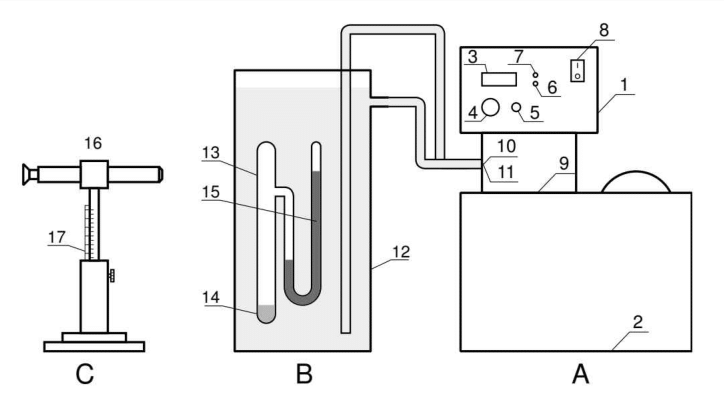
\includegraphics[scale = 0.5]{./images/stand.png}
	\caption{Схема установки}
	\label{fig:stand}
\end{figure}

Установка включает термостат A, экспериментальный прибор B
и отсчетный микроскоп C.

В термостат погружен запаянный прибор 13 с исследуемой жидкостью. Над ней находится насыщенный пар (перед заполнением прибора воздух из него был откачан). Давление насыщенного пара определяется по ртутному манометру. Отсчет показаний манометра
производится при помощи микроскопа.

Описываемый прибор обладает важным недостатком: термометр определяет температуру термостата, а не исследуемой жидкости (или ее пара). Эти температуры близки друг к другу лишь в том случае, если нагревание происходит достаточно медленно.

\section{Приборы и материалы}

В работе используются:

\begin{itemize}
	\item Герметический сосуд, заполненный исследуемой жидкостью;
	\item Отсчетный микроскоп;
	\item Термостат.
\end{itemize}

\section{Обработка результатов}

В данном опыте нам нужно снять зависимость давления насыщенных паров воды от температуры. Погрешность термостата примем равной $0.5$ K, а погрешность манометра $0,05$ mm.
Для метода линеаризации нам потребуются погрешности косвенных измерений:
\begin{equation*}
	\Delta_{1/T} = \frac{\Delta_T}{T^2} = 6\text{E-6 1/K}
\end{equation*}
\begin{equation*}
\Delta_{ln(P)} = \frac{\Delta_P}{P} = 3\text{E-3}
\end{equation*}

Метод конечных разностей заключается в следующем:
\begin{equation*}
	\frac{dy}{dx} \approx \frac{y_{i+1} - y_{i-1}}{x_{i+1} - x_{i-1}}
\end{equation*}

Занесем результаты экспериментов в таблицы, построим графики, найдем угловой коэффициент и погрешность.

\begin{longtable}[H]{|l|l|l|l|} 
	
	\caption{Зависимость давления от температуры при нагревании} 
	
	\\ \hline
	$T$, К & $1/T$, 1/K & $P$, mmHg & $\ln{P}$ \\ \hline
	\endfirsthead
	\hline
	$T$, К & $1/T$, 1/K & $P$, mmHg & $\ln{P}$ \\ \hline
	\endhead
	
	294    & 0.003401   & 19.1      & 2.949    \\ \hline
	295    & 0.003389   & 20.9      & 3.039    \\ \hline
	296    & 0.003378   & 21.8      & 3.081    \\ \hline
	297    & 0.003367   & 22.6      & 3.117    \\ \hline
	298    & 0.003355   & 24.2      & 3.186    \\ \hline
	299    & 0.003344   & 24.9      & 3.214    \\ \hline
	300    & 0.003333   & 26.9      & 3.292    \\ \hline
	301    & 0.003322   & 27.8      & 3.325    \\ \hline
	302    & 0.003311   & 29.6      & 3.387    \\ \hline
	303    & 0.003300   & 31        & 3.433    \\ \hline
	304    & 0.003289   & 33.2      & 3.502    \\ \hline
	305    & 0.003278   & 34.5      & 3.540    \\ \hline
	306    & 0.003267   & 37.3      & 3.618    \\ \hline
	307    & 0.003257   & 38.5      & 3.650    \\ \hline
	308    & 0.003246   & 41        & 3.713    \\ \hline
	309    & 0.003236   & 43.5      & 3.772    \\ \hline
	310    & 0.003225   & 45.2      & 3.811    \\ \hline
	311    & 0.003215   & 47.8      & 3.867    \\ \hline
	312    & 0.003205   & 50.6      & 3.923    \\ \hline
	313    & 0.003194   & 53.6      & 3.981    \\ \hline
\end{longtable}

\begin{figure}[H]
	\centering
	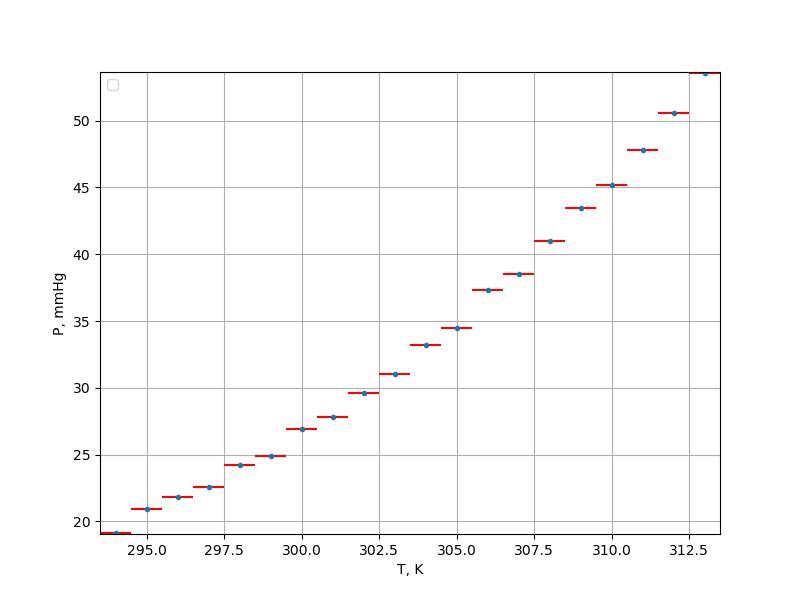
\includegraphics[scale = 0.8]{./images/He.png}
	\caption{Измерения при нагревании. Расчет методом конечных разностей. L = $41 \pm 5\frac{\text{кДж}}{\text{моль}}$ }
\end{figure}

\begin{figure}[H]
	\centering
	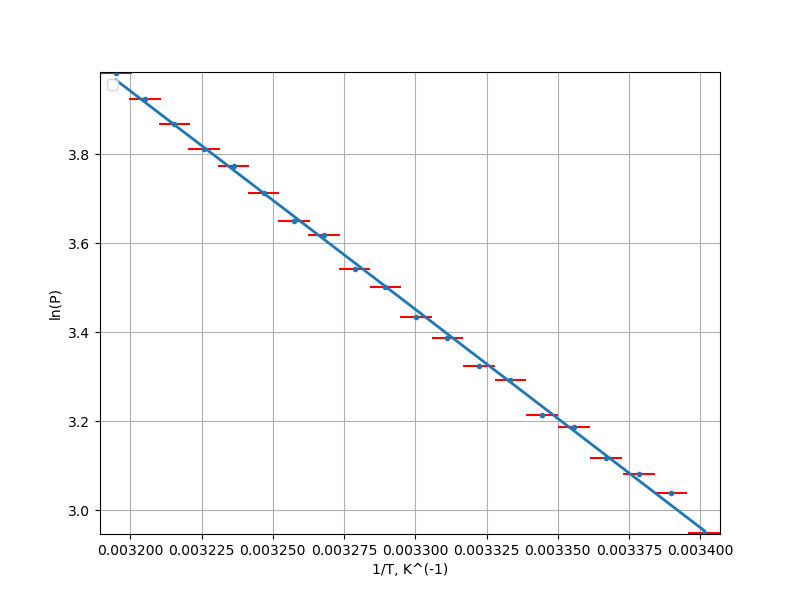
\includegraphics[scale = 0.8]{./images/HeLin.png}
	\caption{Измерения при нагревании. Расчет методом линеаризации. L = $40.7 \pm 0.4\frac{\text{кДж}}{\text{моль}}$ }
\end{figure}



\begin{longtable}[H]{|l|l|l|l|}
	\caption{Зависимость давления от температуры при охлаждении} 
	
	\\ \hline
	$T$, К & $1/T$, 1/K & $P$, mmHg & $\ln{P}$ \\ \hline
	\endfirsthead
	\hline
	$T$, К & $1/T$, 1/K & $P$, mmHg & $\ln{P}$ \\ \hline
	\endhead
	
294    & 0.003401   & 19.5      & 2.970    \\ \hline
295    & 0.003389   & 20.3      & 3.010    \\ \hline
296    & 0.003378   & 21.9      & 3.086    \\ \hline
297    & 0.003367   & 244       & 5.497    \\ \hline
298    & 0.003355   & 24.7      & 3.206    \\ \hline
299    & 0.003344   & 25.8      & 3.250    \\ \hline
300    & 0.003333   & 26.9      & 3.292    \\ \hline
301    & 0.003322   & 28.9      & 3.363    \\ \hline
302    & 0.003311   & 30.3      & 3.411    \\ \hline
303    & 0.003300   & 32        & 3.465    \\ \hline
304    & 0.003289   & 34.5      & 3.540    \\ \hline
305    & 0.003278   & 36.3      & 3.591    \\ \hline
306    & 0.003267   & 38.3      & 3.645    \\ \hline
307    & 0.003257   & 39.3      & 3.671    \\ \hline
308    & 0.003246   & 42.5      & 3.749    \\ \hline
309    & 0.003236   & 44.8      & 3.802    \\ \hline
310    & 0.003225   & 47.2      & 3.854    \\ \hline
311    & 0.003215   & 48.1      & 3.873    \\ \hline
312    & 0.003205   & 51        & 3.931    \\ \hline
313    & 0.003194   & 53.6      & 3.981    \\ \hline
\end{longtable}

\begin{figure}[H]
	\centering
	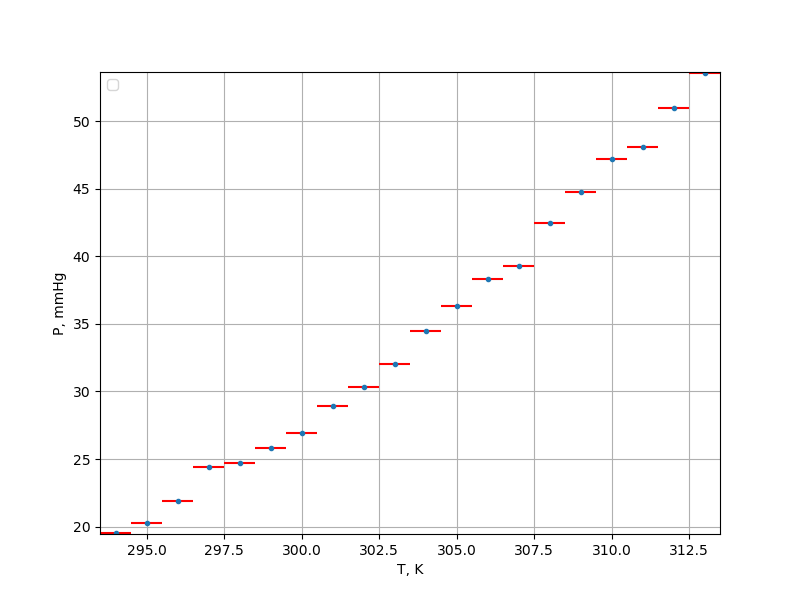
\includegraphics[scale = 0.8]{./images/Co.png}
	\caption{Измерения при охлаждении. Расчет методом конечных разностей. L = $41 \pm 10\frac{\text{кДж}}{\text{моль}}$ }
\end{figure}

\begin{figure}[H]
	\centering
	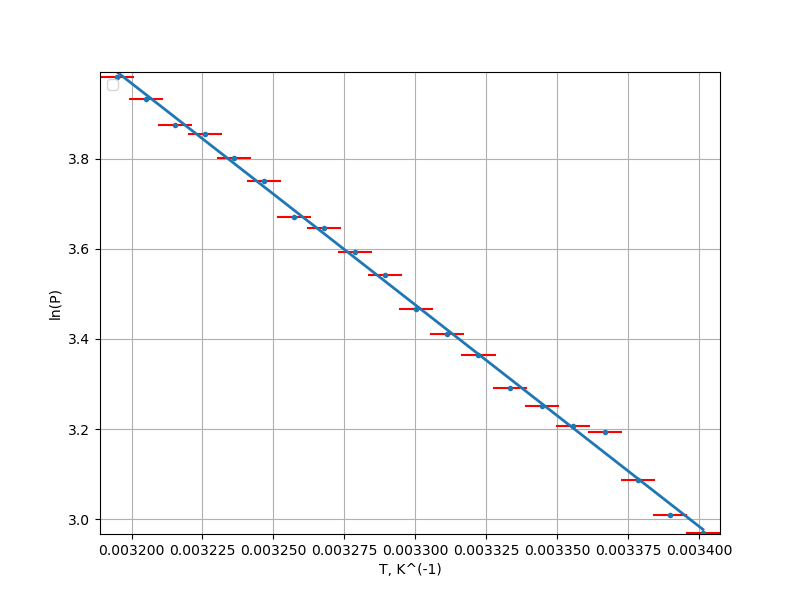
\includegraphics[scale = 0.8]{./images/CoLin.png}
	\caption{Измерения при охлаждении. Расчет методом линеаризации. L = $40.8 \pm 0.5\frac{\text{кДж}}{\text{моль}}$ }
\end{figure}

\section{Вывод}

После обработки результатов можно видеть, что полученное значение теплоты парообразования воды $40.7 \pm 0.4\frac{\text{кДж}}{\text{моль}}$ лежит очень близко к табличному (40680$\frac{\text{Дж}}{\text{моль}}$). Также, можно заметить, что метод линеаризации дает намного большую точность, чем метод конечных разностей (0.98\% и 12.19\% соответственно). 
Увеличение погрешности полученной при обработке измерений 2 эксперимента (в процессе охлаждения) может быть связано с менее равномерным изменением температуры жидкости.

\end{document}